\documentclass[12pt]{article}
\usepackage{amsmath}
\usepackage{grffile}
\usepackage{graphicx}
\usepackage{amsfonts}
\usepackage{pdfpages}
\usepackage{appendix}
\usepackage{parskip}
\renewcommand*{\thesection}{\alph{section}.}

\author{Sundaresan G}
%\title{Advertisement No. CDS/KA/SERB-SRG/DEC2020/RA}
\begin{document}
	
\begin{titlepage}
	\begin{center}
		\vspace*{1cm}
		
		\textbf{\Large{Solution to the 1D Heat Equation}}
		
		\vspace{0.5cm}
		Advertisement No. CDS/KA/SERB-SRG/DEC2020/RA
		
		\vspace{1.5cm}
		
		A report submitted for the application of\\
		Project Assistant Position
		
		
		\vfill
		
		\textbf{\large{Sundaresan G}}\\
		Scientist/Engineer\\
		ISRO Propulsion Complex
		
		\vspace{0.8cm}
		
		B.Tech Mechanical Engineering\\
		Batch of 2016, NITT\\
		
	\end{center}
\end{titlepage}
\tableofcontents

	\section{Analytical Solution}
	Given 
	\begin{equation} \label{heat_eqn}
	 u_t=u_{xx} \,\,,\,\, x\in [0,1] 
	\end{equation}
	subject to periodic boundary conditions 
	\begin{equation*}
	 u(0,t)=u(1,t) \quad \text{and} \quad u_x(0,t)=u_x(1,t)    
	\end{equation*}
	 and initial condition
	 \begin{equation}\label{initial}
	 u(x,0)=\sin(2\pi x).    
	 \end{equation}

	The given problem is a well posed homogeneous linear PDE and has a unique solution for the given boundary and initial conditions. The solution is derived as follows by separation of variables:
	
	Let 
	\begin{equation}
	    u(x,t)=X(x)\,T(t).
	\end{equation}
	Substituting into (\ref{heat_eqn}), we have 
	\begin{equation*}
	    XT_t=X_{xx}T \implies \frac{X_{xx}}{X}=\frac{T_t}{T}=\alpha,
	\end{equation*}
	where $\alpha$ is a constant since the LHS is only a function of $x$ and RHS is a function of $t$. We now examine three cases for $\alpha$:
	
	Case 1: $\alpha=0$
	\begin{equation*}
	        X(x)=ax+b\,\,,\,\, T(t)=c,
	\end{equation*}
	\begin{equation} \label{case1}
	\implies u^{\alpha=0}=a_1 x + a_2.
	\end{equation}
	
	Case 2: $\alpha = \beta^2 > 0$
	\begin{equation*}
	X(x)=ae^{\beta x}+be^{-\beta x}\,\,,\,\, T(t)=ce^{\beta^2 t^2},
	\end{equation*}
	\begin{equation}\label{case2}
	\implies u^{\alpha>0}=(b_1e^{\beta x}+b_2e^{-\beta x})e^{\beta^2 t^2},
	\end{equation}
	where $b_1$ and $b_2$ are arbitrary constants depending on $\beta$.
	
	Case 3: $\alpha = -\lambda^2 < 0$
	\begin{equation*}
	X(x)=a\cos({\lambda x})+b\sin({\lambda x})\,\,,\,\, T(t)=ce^{-\lambda^2 t^2},
	\end{equation*}
	\begin{equation}\label{case3}
	\implies u^{\alpha<0}=(c_1\cos({\lambda x})+c_2\sin({\lambda x}))e^{-\lambda^2 t^2}.
	\end{equation}
	where $c_1$ and $c_2$ are arbitrary constants depending on $\lambda$.
		
	Due to the homogenous and linear nature of the given PDE, a finite sum of (\ref{case1}), (\ref{case2}) and (\ref{case3}) satisfies the PDE. It can be also proved that an infinite convergent sum consisting of (\ref{case1}), (\ref{case2}) and (\ref{case3}) satisfies the PDE. However we would not delve into this topic. For the given problem with the given initial condition, it is enough to consider case 3. Hence, 
	
	\begin{equation}
	u(x,t) = \left(c_1\cos({\lambda x})+c_2\sin({\lambda x})\right)\,e^{-\lambda^2 t^2}.
	\end{equation}	
		
	Applying boundary condition $u(0,t) = u(1,t)$, we get		
	\begin{equation} \label{eq1}
	c_1(\cos({\lambda })-1)+c_2\sin({\lambda}) = 0
	\end{equation} 
	
	Applying boundary condition $u_x(0,t)=u_x(1,t)$ and the fact that $\lambda \neq 0$, we get	
	\begin{equation} \label{eq2}
	c_1\sin(\lambda) + c_2(1-\cos(\lambda))=0 \end{equation}
	
	Solving equations (\ref{eq1}) and (\ref{eq2}), we get the following two equations
	\begin{equation*}
	c_1=c_2=0.
	\end{equation*}
	 The above equation leads to a trivial solution and does not satisfy the given initial condition. Hence the following must hold 
	 \begin{equation*}
	 \sin(\lambda)=(1-\cos(\lambda))=0,
	 \end{equation*}	
	which is satisfied if and only if	
	\begin{equation*}
	\lambda = n \pi, \quad \text{where}\quad  n \in \mathbb{Z}\setminus\{0\}
	\end{equation*}	
	For the given initial condition (\ref{initial}), we get	
	\begin{equation*}
	c_1 = 0,\quad \lambda = 2\pi\quad \text{and} \quad c_2 = 1.
	\end{equation*}
	
	The analytical solution is therefore given by	
	\begin{equation}
	u(x,t)= \sin(2 \pi x)\, e^{-4 \pi^2 t^2}
	\end{equation}
	
	The above solution satisfies the PDE, initial and boundary conditions. Moreover due to well posed nature of the problem, the solution obtained is a unique one (by maximum energy principle).
	
	\section{Numerical Scheme}
	Discretizing (\ref{heat_eqn}) by the explicit Euler (time derivative) and second order central difference (space derivative) scheme, we have
		\begin{equation*}
		u^{t+\Delta t}_{i}= u^t_i + {\Delta t \over (\Delta x)^2} \left(u^t_{i+1}-2u^t_i+u^t_{i-1}\right), \quad \text{where} \quad i=1,\ldots,n-1.
		\end{equation*} 
	
	For $i=0,n$, the discretized equations, with periodic boundary conditions, yield 
	\begin{equation*}
	u^{t+\Delta t}_{0}= u^t_0 + {\Delta t \over \left(\Delta x\right)^2} \left(u^t_{1}-2u^t_0+u^t_{n-1}\right) \quad \text{and}\quad 	u^{t+1}_{n}= u^{t+1}_0 
	\end{equation*} 

	The convergence and stability criteria, 
	\begin{equation*}
	\frac{\Delta t}{\left(\Delta x\right)^2} \leq \frac{1}{2}
	\end{equation*}
	requires $n \leq 223$ for $\Delta t=0.00001$.

	\section{Numerical simulations}
	
	A code is written in C language and given in Appendix A. It uses command line arguments for input of Number of grid points (n) and Time step at which solution is required. Please compile it using a suitable compiler (GCC) as follows	
	\begin{center}
		\begin{tabular}{l}
			\textbf{gcc code.c -o "output file name"} \\
			\textbf{"output file name".exe "n" "Time step(s)"}
		\end{tabular}
	\end{center}
	
	For example,
	
	\begin{center}
		\begin{tabular}{l}
			\textbf{gcc code.c -o results} \\
			\textbf{results.exe 200 300 500 1000}
		\end{tabular}
	\end{center}

	The above example inputs 200 as the number of grid points and prints the numerical and analytical solutions at 300, 500 and 1000 time steps. 

	\textbf{Note:} The maximum number of grid points (default:128) the code accepts is 220 (for convergence) and the maximum time step (default: 0, 100, 500 and 1000) is 3000 and number of time step arguments (default:4) is 10.
	
	\newpage
	
	\section{Solution Plot for 128 grid points}
	
	\begin{figure}[h]
		\centering
	\includegraphics[scale=1.05, angle=90]{"Gnuplot/NSvsAS_plot_for_128_grid_points.eps"}
	\caption{Analytical solution Vs Numerical solution at time steps 0, 100, 500 and 1000}	
	\end{figure}
			
	\newpage
	
	\section{Average Error in the Domain at each time step}
		
	\begin{figure}[h]
		\centering
		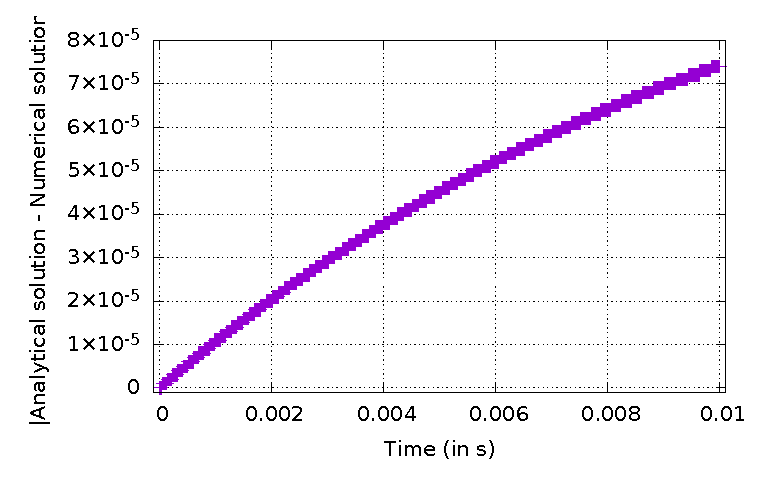
\includegraphics[scale=1.05, angle=90]{"Gnuplot/Error_vs_time_for_128_grid_points.eps"}
		\caption{Average Error(AS-NS) vs Time for 128 grid points}	
	\end{figure}
	

%	\includepdf[scale=0.65,pages=1, angle=90, pagecommand=\section{Solution Plot for 128 grid points}]{"../Gnuplot/NSvsAS_plot_for_128_grid_points.pdf"}
	
		%\includepdf[pages=-]{"D:/iisc project/1d-heat-eqn-solver-single-array/Gnuplot/NSvsAS_plot_for_128_grid_points.pdf"}
%	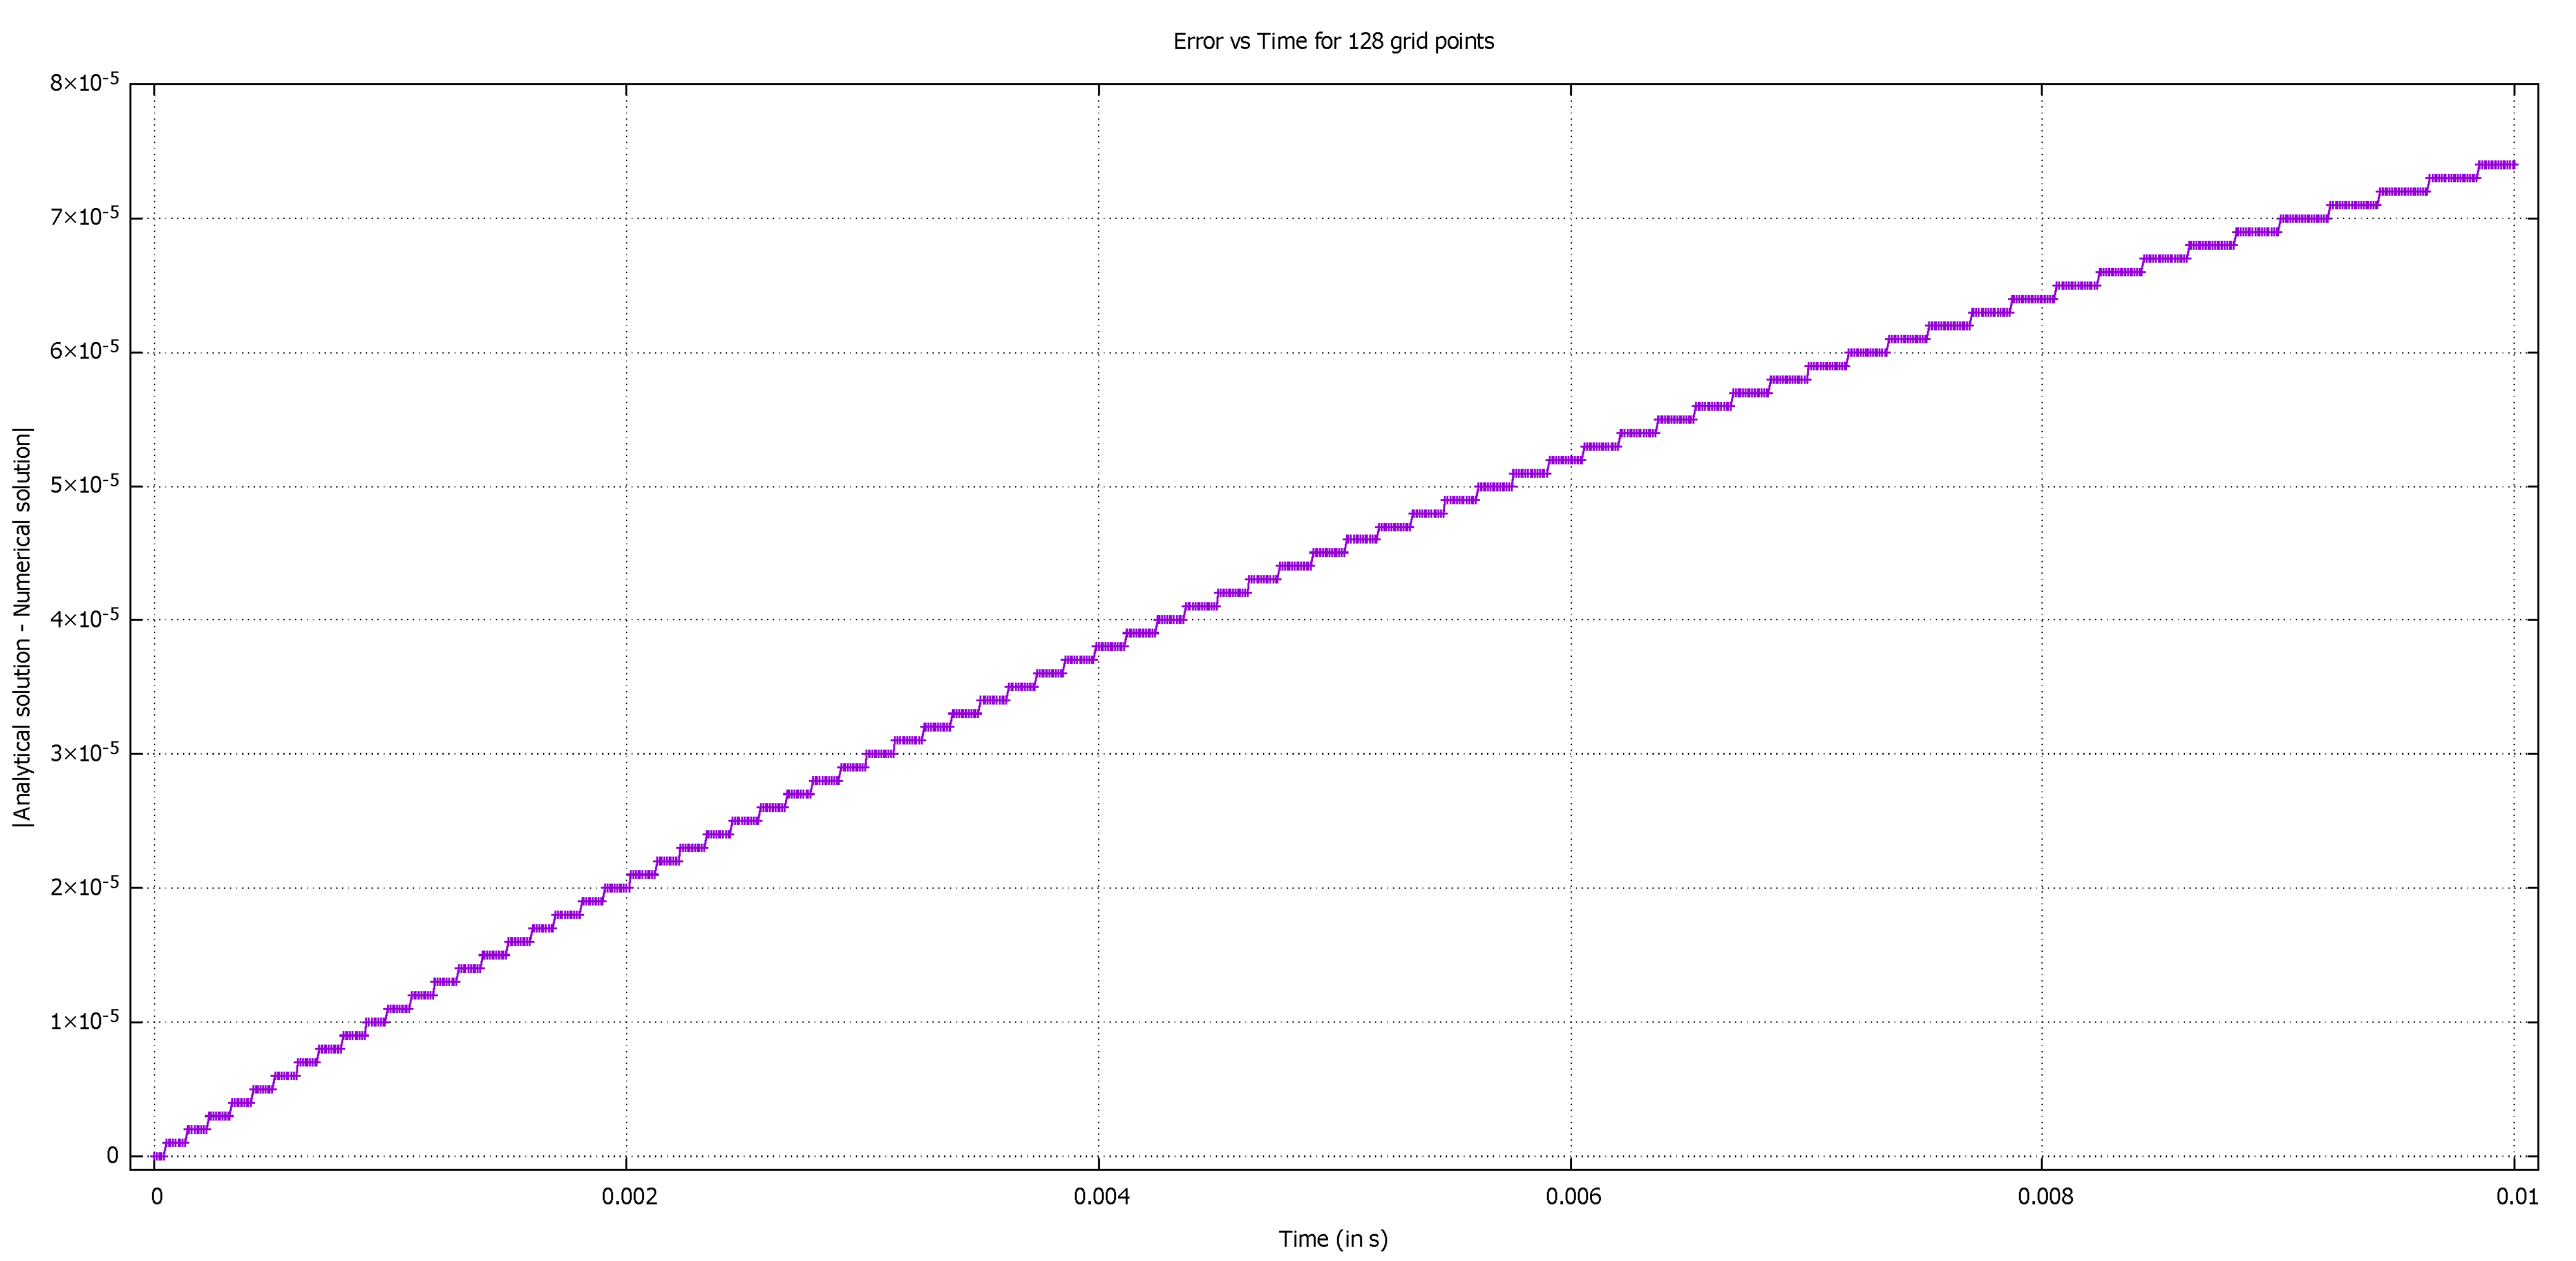
\includepdf[scale=0.65,pages=1,angle=90, pagecommand=\section{Average Error in the Domain at each time step}]{"../Gnuplot/Error vs time for 128 grid points.pdf"}

	\appendix
		
	\includepdf[scale=0.65,pages=1, pagecommand=\section{Appendix A: C code}]{"code.pdf"}
	\includepdf[scale=0.65,pages={2,3}]{"code.pdf"}
	
\end{document}